\section{Client Application}

In the~design chapter~\ref{chapter:design}, the~following technologies were selected for the~client application implementation.
According to the~design, the~implemented application must support web and Windows and other desktop platforms, respectively.
It must also be easily extensible to mobile devices.
Therefore, the~Flutter framework was chosen, enabling cross-platform development on web, desktop, and mobile platforms.
The~Bloc library was chosen for the~state management app state, which, thanks to its asynchronous approach, provides a~robust implementation and allows easy expansion or modification.

\subsection{Used Technologies}

The~Flutter framework in version 2.10.5 was used on its stable channel.
This version uses the~Dart programming in version 2.16.2.
The~package \mintinline{text}|flutter_bloc| in version 8.0.1 was used in the~presentation layer for providing the~Bloc library.
This package provides the~basic implementation of the~Bloc library and supporting widgets and other things for use with the~Flutter framework.

The~package \mintinline{text}|get_it| in version 7.2.0 was used for dependency injection in the~presentation layer.
This package allows registering specific class implementations to their interfaces.
Registered classes are then located from anywhere in the~code.

The~data layer uses the~package \mintinline{text}|http| in version 0.13.4 for the~HTTP communication.
This package provides an~interface for sending HTTP methods POST, GET, PUT, DELETE, etc.

The~business layer uses package \mintinline{text}| shared_preferences| in version 2.0.13 to store the~token.
This package stores data in the~appropriate place based on the~platform.

\subsection{Command Blocks Rendering}

Command blocks are one of the~most critical components of the~implemented game and their implementation, and the~whole development process was fascinating.
These are used for visual programming of individual game missions.
Before describing the~development of this feature, there is a~little reminder of what command blocks are and how they should behave.

Command blocks are used to program a~game mission.
Blocks are visual components that can be grabbed and moved within the~left panel of the~game mission screen.
An example of command blocks is in the~figure~\ref{fig:commandblocks}.
Blocks are part of the~command block list, and if a~player tries to drop a~block outside that list, the~command is deleted.
The~player can use command blocks that are available in the~command block palette.
Command blocks can be dragged to the~command block list from this palette.

\begin{figure}
    \centering
    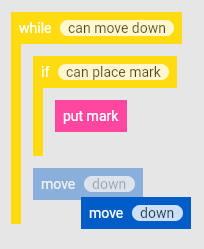
\includegraphics[width=0.4\linewidth]{assets/implementation/commandblocks.png}
    \caption{Command Blocks}
    \label{fig:commandblocks}
\end{figure}

Command blocks use widgets for their implementation.
The~initial idea for the~implementation was to use one of the~already existing widgets of the~Flutter framework.
Flutter contains several widgets that could handle similar functionality, so several options have been tried.

One of the~ways to implement this could be \mintinline{text}|ReorderableListView| widget from the~Flutter Material library.
According to~\cite{a2022_material}, this widget works like a~regular widget that positions its children in a~column, provides scrolling, and allows to drag items within the~list.
This widget provides different drag-and-drop behavior based on whether it's used on a~mobile device where the~player uses a~finger to drag or on a~web where the~player uses a~mouse to drag elements.
All elements of the~list must have a~unique key.
The~\mintinline{text}|ReorderableListView| widget would work well if it did not need to be able to nest command blocks.
However, this widget does not support element nesting, and a~similar solution using this widget failed.
In addition, the~elements in this widget only drag inside their container, which is also not required.
The~elements should be possible to drag in all directions and across different containers or drag elements from the~command block palette.

Another option would be to use the~\mintinline{text}|Draggable| and \mintinline{text}|DraggableTarget| widgets.
These widgets, according to~\cite{a2022_material}, work in their interplay.
Widget \mintinline{text}|Draggable| defines the~data that the~widget should transmit.
This widget also has three children that differentiate what the~widget should look like, what the~widget should look like when dragged, and how the~area behind the~widget should look.
The~second widget, widget \mintinline{text}|DraggableTarget|, is used to determine where \mintinline{text}|Draggable| widget can be dragged.
It defines several functions according to which the~widget determines whether the~dragged widget should be accepted or what should happen if dropped.
It also defines a~builder that determines how the~widget should appear based on whether or not any data has been dragged to it.
This approach sounded very promising at first; however, it turned out that it would be complicated to use these widgets to make a~dynamic implementation within the~scope of command block requirements.
One problem was that if a~new command block was added to the~end of the~command block list, a~new slot for the~next block needed to be created.
It would also be challenging to implement block reordering.
Additional empty \mintinline{text}|DraggableTarget| widgets would have to be added to all the~used \mintinline{text}|DraggableTarget| widgets to check if the~player moves the~block to one of the~locations between blocks.
After moving the~block, a~recalculation would have to follow, and a~similar situation would be repeated.

Command blocks must be rendered declaratively because widgets in the~Flutter framework are rendered declaratively.
Because the~position of all blocks would have to be complicatedly mapped to the~state, the~second proposed option could not be implemented.
Because of this, a~custom solution was created.
The~solution contains two essential elements, containers, and blocks.
A container is a~widget that will accept blocks.
And blocks are widgets that represent commands.
Some blocks also contain a~nested container to which the~exact definition applies.
In addition, this container and block structure is defined by a~state, which is represented as a~command tree structure.
These commands are of two basic abstract types and can be group or single commands.
Each command has its class that extends one of these abstract classes.
A special case is the~root command class, which is used as the~root of the~tree structure.
That makes a~declarative rendering of the~structure.
It uses its widget \mintinline{text}|CommandItem|, to which an~instance of the~command is passed as an~argument, and according to its abstract type, other \mintinline{text}|CommandItem| widgets are recursively added to the~widget tree.
These \mintinline{text}|CommandItem| widgets then add the~widget \mintinline{text}|CommandBlock| to the~structure, which solves the~visual rendering of the~command block, i.e., displays the~colored rectangle of the~command.
The~entire display of list command blocks takes place in the~\mintinline{text}|CommandsView| widget.

The~moving command blocks feature is missing to complete the~required functions.
For \mintinline{text}|CommandBlock| widget to drag, the~player must hold and move it.
As the~player drags the~block, the~\textquote*{shadow} (as can be seen in the~figure~\ref{fig:commandblocks}) of the~original block must remain beneath it, which moves to the~location where the~block could be placed as it is being dragged.
It must also be determined in which specific container this block is to be placed.
Whether in the~main or in one of the~nested, which belong to the~commands that have nested blocks.
If the~block is moved outside of any container, the~\textquote*{shadow} will soften, indicating that it will be removed if the~player releases the~block.
Conversely, the~block must also be able to be moved and copied from the~command palette.
All these operations continuously update the~state of the~command tree structure.
The~blocks themselves are not physically moved.
The~state according to which the~widgets are redrawn changes.
The~\mintinline{text}|Key| keys are used to ensure that the~framework does not redraw blocks that do not change or that the~algorithm knows which widget to move.
Keys are, according to~\cite{a2022_material}, unique widget identifiers.
The~key for the~\mintinline{text}|CommandItem| widget is an~\mintinline{text}|ObjectKey| key using the~object of the~respective command, i.e., its hash.

The~move is processed in the~\mintinline{text}|CommandsView| widget.
All blocks and containers are registered in this widget so that this widget can subsequently browse them.
To start a~move event, the~\mintinline{text}|CommandBlock| widget (which draws a~visual rectangle) uses the~\mintinline{text}| Listener| widget, which according to~\cite{a2022_material} provides an~interface to basic pointer events.
Specifically, the~\mintinline{text}|PointerDownEvent| event is captured.
This event is passed to the~\mintinline{text}|CommandsView| widget, which starts processing the~move.
It also starts listening to other events using the~Flutter class \mintinline{text}|PanGestureRecognizer|.
It provides an~interface for capturing update and end events.
Widget \mintinline{text}|CommandsView| uses the~\mintinline {text}|Stack| widget, which allows to display widgets on top of each other.
It will display a~special proxy widget at the~top of this stack.
Visually, this widget is the~original widget being dragged.
However, as described above, the~original widget remains in place as a~\textquote*{shadow.}
This added proxy widget is the~one that is being dragged.

For each update event, the~position of the~proxy widget must be updated by the~delta difference of the~event.
Subsequently, a~lookup is performed to find the~nearest container in which the~event position is located, i.e., the~player's pointer.
If no container is found, the~dragged command bloc is marked as suitable for deletion.
If found, the~block closest to the~dragged block is also found.
That determines the~position to which the~block's \textquote*{shadow} should move.
The~state is updated, and Flutter declaratively redraws the~command blocks, so the~\textquote*{shadow} visually moves to the~correct position.

Iteration through all registered containers is used for the~lookup of the~nearest container.
The~current container's \mintinline{text}|RenderObject| or \mintinline{text}|RenderBox|, respectively, is requested using \mintinline{dart}|final containerRender = container.context.findRenderObject() as RenderBox;|.
Then, as can be seen in the~code~\ref{listing:closest-container}, the~position of the~container is compared with the~cursor position, and then, if the~container is not part of a~block (that is if the~container is not a~block subcommand), the~nearest such container is found.
A similar algorithm finds the~nearest block below.

\begin{listing}
    \caption{Closest Container Lookup}
    \label{listing:closest-container}
    \begin{minted}{dart}
if (containerRender.size.contains(
    position 
        - containerRender.localToGlobal(Offset.zero) 
        + const Offset(2, 2)
)) {
    // But it is not subtree of original item.
    if (!container._isChildOfItem(_dragging!)) {
        // Find the closest one.
        if (container.index.length > maxIndexes) {
            maxIndexes = container.index.length;
            closestContainer = container;
        }
    }
}
    \end{minted}
\end{listing}

Some blocks may have conditions or directions.
These are also rendered by the~\mintinline{text}|CommandBlock| widget if the~command has a~choice of condition or direction.
An overlay must be created when the~mouse is moved over for a~player to be able to select a~condition or direction in such a~block.
The~options are displayed in the~respective overlay, and after selecting the~option, the~command state is adjusted.

\subsection{Overlays}

The~custom widget \mintinline{text}{OverlayButton} is used to implement overlays.
This widget is used to select conditions and directions for command blocks in the~game mission and for some submenu buttons in the~menu.

\begin{figure}
    \centering
    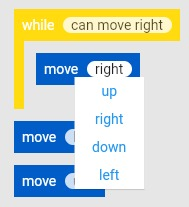
\includegraphics[width=0.4\linewidth]{assets/implementation/overlay.jpeg}
    \caption{Overlay}
    \label{fig:overlay}
\end{figure}

Overlays display content above the~standard widget tree.
Such logic could be created using a~custom implementation using the~\mintinline{text}|Stack| widget.
Implementing it this way for all applications can be annoying and error-prone.
Flutter provides the~\mintinline{text}|Overlay| widget, which implements exactly this functionality.
This can be used to display input suggestions, tooltips, or anything that needs to float above the~screen.
According to~\cite{a2022_material}, \mintinline{text}|Overlay| is \textquote{A stack of entries that can be managed independently.}
\mintinline{text}|Overlay|, therefore, maintains its \mintinline{text}|Stack| and manages widgets that are added to it.
This widget can be created directly, or it can be used already pre-created one using the~\mintinline{text}|Navigator|.
An example of an~overlay for a~command block can be seen in the~figure~\ref{fig:overlay}.

To create an~overlay, the~\mintinline{text}|insert()| method needs to be called on the~mentioned \mintinline{text}|Overlay| created by \mintinline{text}|Navigator|.
\mintinline{text}|OverlayEntry| is used as an~argument for this method.
According to~\cite{a2022_material}, \mintinline{text}|OverlayEntry| is the~object that \mintinline{text}|Overlay| use to represent its items.

In addition, the~custom \mintinline{text}|OverlayButton| widget, which is used for overlays in the~game mission, menu, etc., detects if the~overlay overflows the~screen to the~right or left and adjusts it to be at its edge instead.
Because in some cases, it is necessary to ensure that the~overlay moves with the~widget that triggered it.
For example, when scrolling, it is necessary to synchronize the~position on the~screen.
It can also be used only to synchronize the~position, whether it will change later.
That can be implemented manually, but Flutter has ready functionality for this.
Flutter provides the~ability to create a~\mintinline{text}|LayerLink| object that allows linking a~follower to a~target~\cite{a2022_material}.
\mintinline{text}|OverlayEntry| can use the~\mintinline{text}|CompositedTransformFollower| widget to set the~follower and \mintinline{text}|CompositedTransformTarget| to set the~target.
The~follower will automatically follow the~position of the~target.
\mintinline{text}|OverlayButton| detects enter and end events on the~widget and displays the~overlay accordingly.

\subsection{Networking}

The~\mintinline{text}|http| package is used for networking.
The~package is used to communicate with the~Web API server.
From there, JSON encoded data are fetched.
Fetched data are decoded into \mintinline{text}{Map<String, dynamic>} data and are further processed to create entities.
Most of the~entities has a~factory constructor \mintinline{text}|.fromJson(Map<String, dynamic> json)|.
These constructors parse the~typed JSON and create entities from it.
A simple example of the~user entity can be seen in the~code~\ref{listing:fromjson}.

\begin{listing}
    \caption{From-Json Factory Constructor}
    \label{listing:fromjson}
    \begin{minted}{dart}
factory User.fromJson(Map<String, dynamic> json) {
    return User(
        id: json['id'],
        name: json['name'],
        username: json['username'],
        email: json['email'],
        description: json['description'],
    );
}
    \end{minted}
\end{listing}

Data are usually simple to parse.
There are some compelling cases in which the~parsing is more complicated.
After loading a~game mission, a~\mintinline{text}|GameMission| entity is created.
This entity contains all its properties as simple data types.
But it contains the~\mintinline{text}|commands| and \mintinline{text}|commandsInitial| properties that contains a~string with a~encoded JSON structure.
This structure must be further decoded and processed.
That is done by the~\mintinline{text}|GameMission|'s \mintinline{text}|parseGame()| method.
This method decodes the~command's properties to the~JSON map and recursively creates a~commands tree using the~factory constructor of the~\mintinline{text}|RootCommand|.
This constructor parses its data which are recursively parsed to the~specific command classes.
This process, therefore, elegantly creates a~command tree structure.

\subsection{Router and Navigation}

Flutter initially used an~imperative approach to routing and navigation.
According to~\cite{ryan_2020_navigator}, this was problematic, and it was challenging to push or pop several screens or otherwise change the~state of the~screen stack.
A new Navigator 2.0 API has been added to Flutter, allowing control of the~navigator declaratively.
A schema of Navigator 2.0 can be seen in the~figure~\ref{fig:navigator}.
According to~\cite{kietay_2021_navigator}, the~imperative approach can get the~application into trouble because it does not separate app logic from the~UI logic.
UI logic is separated from app logic using a~declarative approach.
UI logic displays screens according to data, respectively depending on the~application's state.
And app logic retrieves data and changes the~state of the~application.

\begin{figure}
    \centering
    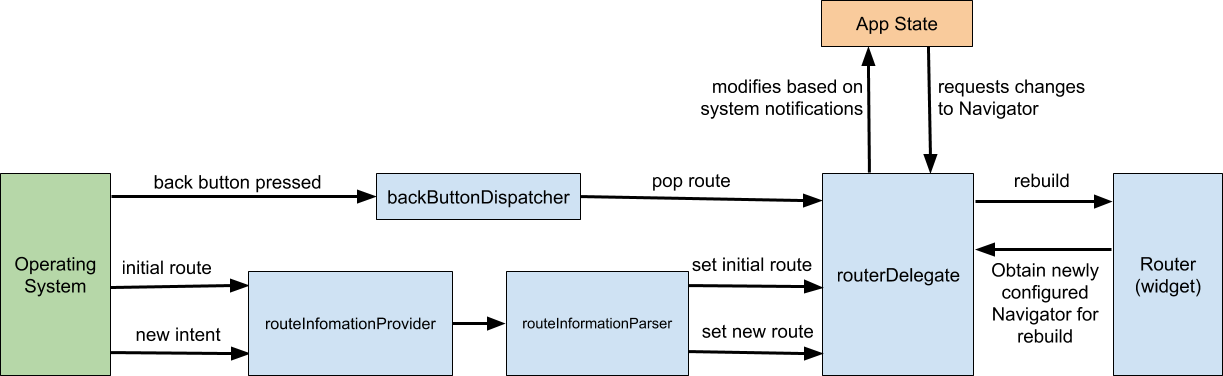
\includegraphics[width=1\linewidth]{assets/implementation/navigator.png}
    \caption{Navigator 2.0~\cite{ryan_2020_navigator}}
    \label{fig:navigator}
\end{figure}

According to~\cite{kietay_2021_navigator}, Navigator 2.0 needs to do three things.
Convert app state to navigator state (build method).
Convert app state to Abstract Data Type (ADT) and further to the~path.
And convert the~path to the~ADT and then to the~app state.
According to~\cite{ryan_2020_navigator}, two new classes are used for this.
The~\mintinline{text}|RouteInformationParser| class, which uses the~\mintinline{text}|parseInformationRouter| to convert the~path to the~ADT and uses the~\mintinline{text}|restoreRouteInformation| method to convert the~ADT to the~path.
And the~\mintinline{text}|RouterDelegate| class, which uses the~\mintinline{text}|setNewRoutePath| to convert the~ADT to app state and the~\mintinline{text}|currentConfiguration| method to convert app state to the~ADT.

Several screens have been created for the~implemented game, each of which must have an~appropriate representation using a~path, navigation state, and app state.
According to the~text above, the~Bloc library is used as the~app state, which represents the~app state.
Of course, this state is only in the~context of routing.
It contains several states (and therefore screens) that can extend interfaces.
Interface \mintinline{text}|RequiresAuthentication| is used to indicate those states that require the~user to be able to access them only when logged in.
This Bloc, therefore, communicates with the~Bloc that manages the~authentication.
Before Bloc invokes a~state redirecting to a~given screen, it checks that the~user is signed in if the~future state implements this interface.
It also contains the~\mintinline{text}|ForbiddenAfterAuthentication| interface, which works very similarly to the~former.
If the~user tries to get to the~screen, they will be redirected to the~sign-in screen instead.
The~difference is that Bloc will not emit those states that redirect to that screen if the~user is signed in.
That is used for sign-in and sign-up screens that are only available to anonymous users.
If the~user still tries to get to the~screen, they will be redirected to the~home screen.
The~scheme of individual states and their attributes can be seen in the~figure~\ref{fig:routing}.

\begin{figure}
    \centering
    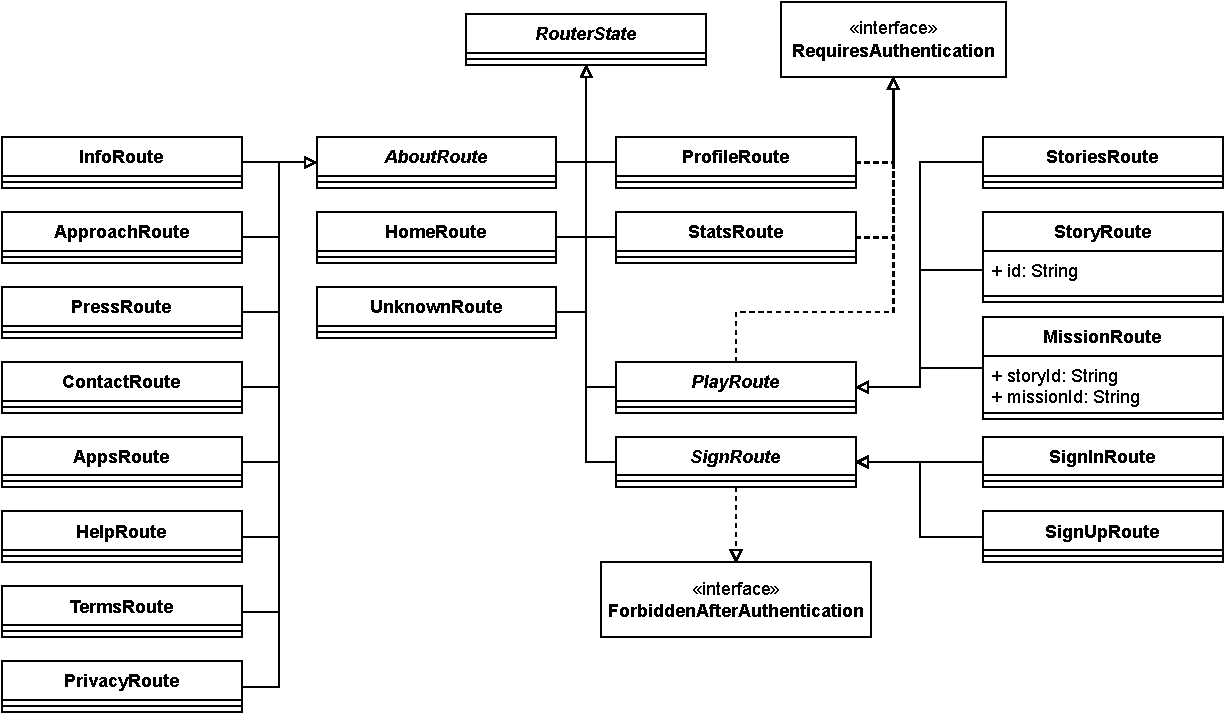
\includegraphics[width=1\linewidth]{assets/implementation/routing.pdf}
    \caption{Routing}
    \label{fig:routing}
\end{figure}

\subsection{Game Processing}

At the~beginning of this section, command blocks were described as one of the~critical components of the~implemented game.
Game missions consist of two critical parts.
One is the~part with the~visual programming, wherewith the~help of command blocks, the~player sorts blocks so that the~robot performs the~correct sequence of steps and fulfills the~mission goal.
The~second part is the~game processing.
That includes both game grid implementation, visual representation of the~game state, and processing of visual programming (command blocks).

\begin{figure}
    \centering
    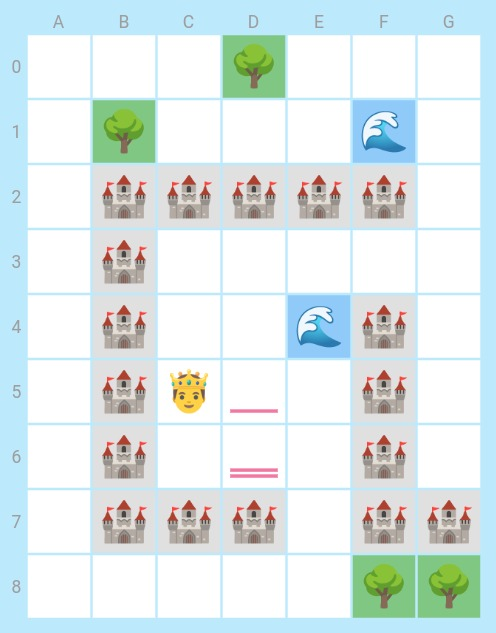
\includegraphics[width=0.5\linewidth]{assets/implementation/gamegrid.jpeg}
    \caption{Game Grid}
    \label{fig:gamegrid}
\end{figure}

The~game grid is implemented as a~grid of cells.
It can be seen in the~figure~\ref{fig:gamegrid}.
These, like command blocks, use widgets to render.
These widgets are rendered into several types according to the~type of each cell.
A walkable cell is rendered as an~empty cell that a~robot can walk on.
This cell can also have several marks.
These appear as horizontal plates.

Several types of non-walkable cells are implemented.
These are walls, forests, and water.
The~wall has a~gray coloration and represents, for example, the~castle walls.
The~forest has a~green coloration and represents an~impenetrable forest.
Water has a~blue tint and represents water.
The~robot must not get out of the~walkable cells.
If a~player tries to step outside the~walkable cell or the~grid, the~game will allow them to see their mistake visually in the~first step.
After this step, however, the~game opens a~failed game dialog, where it reports error.
That can be seen in the~figure~\ref{fig:gamedialog}.
Coordinates with numbers for the~vertical axis and letters for the~horizontal axis are displayed around the~grid.
The~coordinates are also displayed when you hover over a~cell to make navigation easier when thinking about how to complete the~game.

\begin{figure}
    \centering
    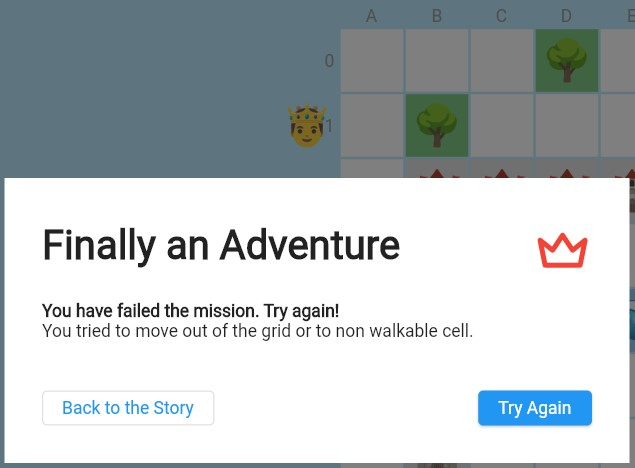
\includegraphics[width=0.7\linewidth]{assets/implementation/gamedialog.jpeg}
    \caption{Game Dialog}
    \label{fig:gamedialog}
\end{figure}

In order for the~player to know clearly where they are in each step, the~robot is marked on the~grid with a~figure with a~crown.
As the~game progresses, this character moves around the~grid to perform the~tasks assigned by the~visual programming.
At the~same time, the~currently executed command block is indicated by an~arrow.
In this way, the~player knows which command is currently being executed and which is responsible for potential unplanned behavior.

After clicking the~play button, the~current command blocks are saved, and an~event to play the~game is added with those commands.
The~game itself is processed in the~\mintinline{text}|processGame()| method in class \mintinline{text}|GameService|, or rather in its implementation class \mintinline{text}|GameServiceImpl|.
This method receives as an~argument an~entity with all the~game data.
The~algorithm thus has access to all the~necessary data.
The~output of this method is the~queue of the~\mintinline{text}|ProcessGameResult| object.
This object contains the~object with the~game and the~index of the~currently processed command.
If an~error occurred in the~given step, the~type of an~error is also included. 
The~algorithm first determines if the~commands are valid.
That is checked by recursively passing commands using their \mintinline{text}|isValid()| method.
If the~commands are valid, the~commands begin to be processed recursively.
The~algorithm gradually calls group and single command processing methods according to the~given command type.

For the~single command type, the~process is trivial.
The~algorithm creates a~clone of the~game object modified by the~given command effect.
Then it is added to the~queue.
If an~error occurs during processing, an~error is also added to it.

For the~group command type, the~command \mintinline{text}|if| is processed separately from the~\mintinline{text}|while| command.
Both commands first add a~state to the~queue, pointing to the~index of their command block.
Command \mintinline{text}|if| then it checks the~condition and, if it is met, it calls the~method to process the~nested commands.
Command \mintinline{text}|while| works similarly, but the~condition is checked in a~while loop.
During this pass, the~\mintinline{text}|speed| argument is counted, which indicates the~number of executed commands of the~given command, i.e., the~method call for solving a~group or single command.

The~\mintinline{text}|size| argument is also calculated at the~beginning of processing, which indicates the~number of blocks used.
The~\mintinline{text}|countSize()| method is invoked over the~root command object.
After the~recursive processing is completed, the~last state is added to the~queue with the~game modified by filled \mintinline{text}|size| and \mintinline{text}|speed| attributes, and the~\mintinline{text}|completed| attribute, which indicates whether the~game was completed.
This is detected by calling the~\mintinline{text}|isCompleted()| method on the~game object.
